\section{What cross-attention shows (post hoc)}\label{sec:resATTN}
The test generations saved, for every canonical image, the cross-attention map of each constraint word at all 40 steps. That gives \atFiles{} maps on \atScenes{} scenes: guidance $w\in\{2,5,7.5,10,15\}$ for the main benchmark and $w=7.5$ for the size family, all at 40 steps. No maps exist for 20-step images, restart branches, prompt switches or the CAG arms, so attention cannot be compared across schedules. All analyses below are post hoc. They use $16\times16$ maps, each word's map normalised to unit mass at every step. \emph{Localisation} is the share of a noun's mass in its top 10\% of cells, and \emph{overlap} is the histogram intersection with the other object nouns of the prompt.

\paragraph{Attention separates found from missed objects from the first steps.} At $w=7.5$ we compare, within the same scene and object, seeds in which the judge found the object with seeds in which it did not (\atPairs{} scene--object pairs in \atPairScenes{} scenes; Figure~\ref{fig:attn-sf}a,b). The noun's attention is more localised and overlaps less with the other nouns when the object is later found. Both differences are distinguishable from zero from the first step; at step 10 they are \atLocTen{} (CI $[\atLocTenLo,\atLocTenHi]$) and \atOvlTen{} ($[\atOvlTenLo,\atOvlTenHi]$). This is a within-scene association, not a causal effect: the initial noise fixes both the early attention layout and, often, the outcome. It is consistent with object neglect being visible early in attention \citep{chefer2023attend} and with forecasting final quality from early attention \citep{diffusionprobe2026}. Figure~\ref{fig:attn-examples} in the appendix shows three pairs chosen by a fixed rule (the three lowest scene identifiers with a two-object prompt and both outcomes; the lowest-index seed of each outcome).

\paragraph{Guidance separates the nouns.} On identical initial noise (same scene, seed and object), higher guidance lowers the overlap between object nouns throughout the trajectory. At step 10 overlap falls from \atOvlTwoTen{} at $w=2$ to \atOvlFifteenTen{} at $w=15$; the paired difference is \atOvlDiffTen, CI $[\atOvlDiffTenLo,\atOvlDiffTenHi]$ (Figure~\ref{fig:attn-sf}c). Over the same range the share of objects found rises from \atDetTwo{} to \atDetFifteen. Figure~\ref{fig:attn-evolution} shows one scene, chosen by rule as the lowest-identifier binding scene with maps at all three scales. At $w=2$ the two nouns' maps stay mixed and the bottle is not drawn; at $w=7.5$ and $15$ they separate within the first ten steps.
\begin{figure}[t]\centering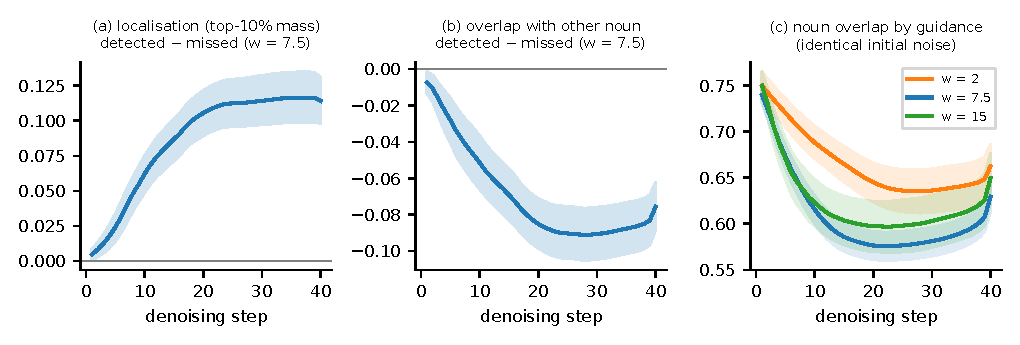
\includegraphics[width=\linewidth]{figures/attn_success_failure.pdf}
\caption{\textbf{Partial test split, post hoc.} (a,b)~Within-scene difference, found minus missed, in a noun's attention localisation and in its overlap with the other nouns at $w=7.5$ (\atPairs{} scene--object pairs, \atPairScenes{} scenes). (c)~Noun overlap at three guidance scales on identical initial noise. Bands: 95\% scene-bootstrap intervals.}\label{fig:attn-sf}\end{figure}
\begin{figure}[t]\centering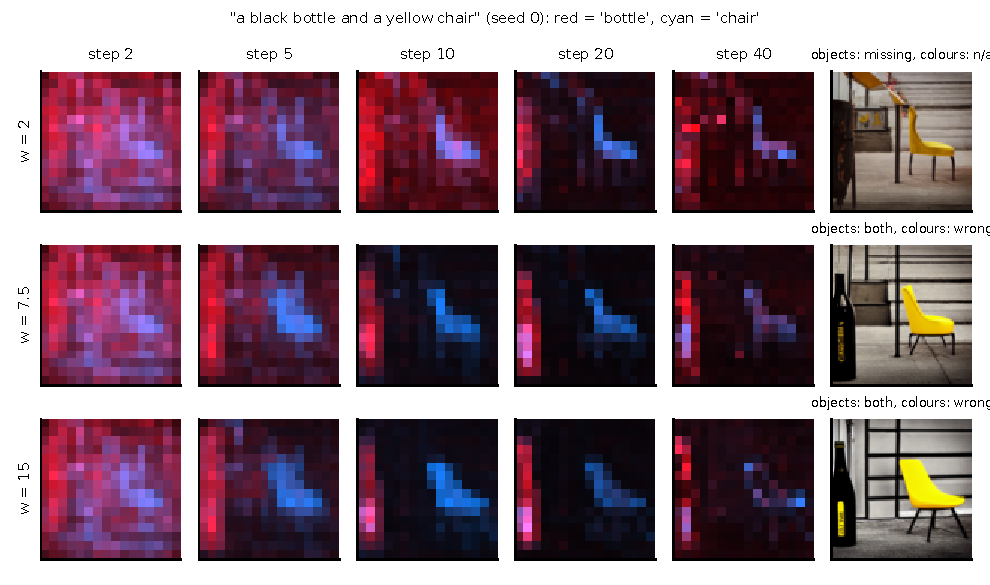
\includegraphics[width=0.92\linewidth]{figures/attn_evolution.pdf}
\caption{\textbf{Illustration, not evidence.} Attention of the two object nouns (red, cyan) at five denoising steps for one prompt and seed at three guidance scales (same initial noise), with the judged outcome. Selection rule: the lowest-identifier binding scene whose seed-0 maps exist at $w=2$, $7.5$ and $15$.}\label{fig:attn-evolution}\end{figure}

\paragraph{Why attention stabilisation does not order the constraint types (HF).} The registered statistic, the step $t_{\mathrm{stab}}$ at which a type's attention signal has travelled half of its total path, does not order types the way restart persistence does (Figure~\ref{fig:attn-tstab}a).
\begin{itemize}
\item At $w=7.5$, $t_{\mathrm{stab}}$ spans only \atTsRangeLo{}--\atTsRangeHi{} steps across types, against 6--20 for $t_{50}$.
\item Binding is the type with the earliest stabilisation (\atTsBind) and the latest persistence (\rbTestBind).
\item The binding signal is the colour word's attention map, which largely follows the object's location. Its stabilisation (\atTsBind) is close to that of presence (\atTsPres) at every guidance scale. The signal therefore records where the colour will be placed, not whether the colour--object assignment has been made.
\end{itemize}
Attention does, however, respond to guidance in the same direction as persistence. Between $w=2$ and $w=15$, $t_{\mathrm{stab}}$ moves earlier by \atTsDiffPres{} steps for presence (paired CI $[\atTsDiffPresLo,\atTsDiffPresHi]$) and by \atTsDiffBind{} for binding, but only by \atTsDiffCount{} for count (Figure~\ref{fig:attn-tstab}b). For presence this is the same direction and a similar size as the HD restart contrast. The two signals agree on \emph{what guidance does}, yet disagree on \emph{which constraint settles first}. This is the pattern expected if attention tracks spatial layout rather than attribute binding.
\begin{figure}[t]\centering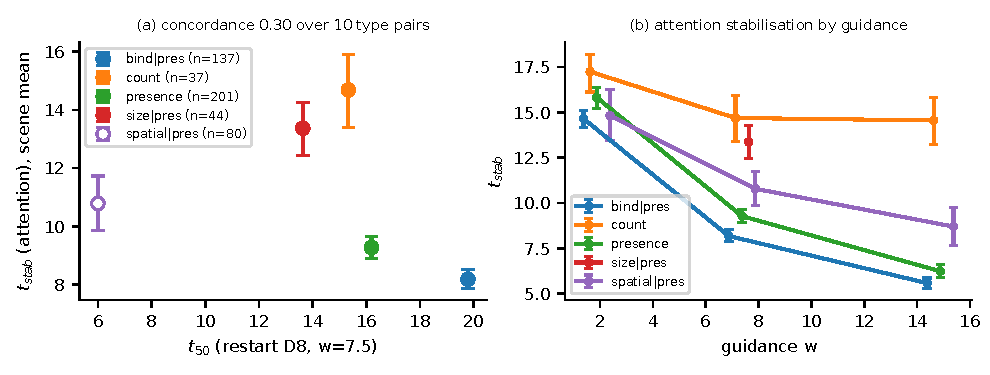
\includegraphics[width=\linewidth]{figures/attn_tstab.pdf}
\caption{\textbf{Partial test split; (a) registered quantities, (b) post hoc.} (a)~Attention stabilisation $t_{\mathrm{stab}}$ (scene means, 95\% intervals) against restart persistence $t_{50}$ per type at $w=7.5$; open marker: left-censored $t_{50}$. (b)~$t_{\mathrm{stab}}$ per type at three guidance scales.}\label{fig:attn-tstab}\end{figure}
